

\documentclass[]{emulateapj}
\usepackage{amsmath}

\usepackage[breaklinks,colorlinks,citecolor=blue,linkcolor=blue]{hyperref}
%urlcolor=
%
\usepackage{etoolbox}

\makeatletter

% Patch case where name and year are separated by aysep
\patchcmd{\NAT@citex}
  {\@citea\NAT@hyper@{%
     \NAT@nmfmt{\NAT@nm}%
     \hyper@natlinkbreak{\NAT@aysep\NAT@spacechar}{\@citeb\@extra@b@citeb}%
     \NAT@date}}
  {\@citea\NAT@nmfmt{\NAT@nm}%
   \NAT@aysep\NAT@spacechar\NAT@hyper@{\NAT@date}}{}{}

% Patch case where name and year are separated by opening bracket
\patchcmd{\NAT@citex}
  {\@citea\NAT@hyper@{%
     \NAT@nmfmt{\NAT@nm}%

\hyper@natlinkbreak{\NAT@spacechar\NAT@@open\if*#1*\else#1\NAT@spacechar\fi}%
       {\@citeb\@extra@b@citeb}%
     \NAT@date}}
  {\@citea\NAT@nmfmt{\NAT@nm}%

\NAT@spacechar\NAT@@open\if*#1*\else#1\NAT@spacechar\fi\NAT@hyper@{\NAT@date}}
  {}{}

\makeatother
%
\usepackage{xspace}
%
\usepackage{apjfonts}
\usepackage{amssymb, amsmath} % for e.g. \lesssim
\usepackage{natbibspacing, natbib}
\usepackage{aas_macros} % for understanding Journal in bib
\usepackage{graphics,graphicx}
%
\newcommand{\vdag}{(v)^\dagger}
\newcommand{\myemail}{tleung@astro.cornell.edu}
\newcommand{\Msun}{\mbox{M$_{\odot}$}\xspace}
\newcommand{\Rsun}{\mbox{R$_{\odot}$}\xspace}
\newcommand{\Lsun}{\mbox{L$_{\odot}$}\xspace}
\newcommand{\LIR}{\mbox{$L_{\rm IR}$}\xspace}
\newcommand{\LFIR}{\mbox{$L_{\rm FIR}$}\xspace}
%
\newcommand{\rarr}{$\rightarrow$}
\newcommand{\aco}{\mbox{CO($J$\,=\,1\,\rarr\,0) }}
\newcommand{\bco}{\mbox{CO($J$\,=\,2\,\rarr\,1) }}
\newcommand{\cco}{\mbox{CO($J$\,=\,3\,\rarr\,2) }}
\newcommand{\rot}[3][CO]{\mbox{#1($J$\,=\,#2\,\rarr\,#3)}}
%
\newcommand{\alphaco}{$\alpha_{\rm CO}$}
\newcommand{\cii}{[C{\scriptsize II}]}
\newcommand{\Lp}[1][CO]{\mbox{$L^{\prime}_\textrm{\fontsize{8pt}{12pt}\selectfont{#1}}$}}
\newcommand{\kms}{km\,s$^{-1}$\xspace}
\newcommand{\LpU}{\mbox{K\,\,km\,\,s$^{-1}$\,\,pc$^2$}\xspace}
\newcommand{\pmOne}{\mbox{$^{-1}$}\xspace}
% Numerical values
\newcommand{\E}[1]{$\times10^{#1}$}
\newcommand{\petm}[2]{$^{+#1}_{-#2}$}
%
\newcommand{\eg}{{e.g.,~}}
\newcommand{\ie}{{i.e.,~}}
%
\newcommand{\Fig}[1]{Figure~\ref{fig:#1}}
\newcommand{\Eq}[1]{Equation~\ref{eq:#1}}
\newcommand{\Tab}[1]{Table~\ref{tab:#1}}
\newcommand{\Sec}[1]{\S\ref{sec:#1}}
%
\newcommand\tna{\,\tablenotemark{a}}
\newcommand\tnb{\,\tablenotemark{b}}
\newcommand\tnc{\,\tablenotemark{c}}
\newcommand\tnd{\,\tablenotemark{d}}
\newcommand\tne{\,\tablenotemark{e}}
\newcommand\tnf{\,\tablenotemark{f}}
\newcommand\tng{\,\tablenotemark{g}}
\newcommand\tnh{\,\tablenotemark{h}}
\newcommand\tni{\,\tablenotemark{i}}
\newcommand\tnj{\,\tablenotemark{j}}
\newcommand\tnk{\,\tablenotemark{k}}
\newcommand\tnl{\,\tablenotemark{l}}
%
\def\herschel {{\it Herschel Space Observatory}\xspace}
\def\alma     {Atacama Large (sub-)Millimeter Array (ALMA)\xspace}
\def\spitzer {{\it Spitzer Space Observatory}\xspace}
\def\pdbi     {Plateau de Bure Interferometer\xspace}
\def\carma    {Combined Array for Research in Millimeter-wave Astronomy\xspace}
\def\cso      {Caltech Sumillimeter Observatory (CSO)\xspace}
\def\noema    {Northern Extended Millimeter Array (NOEMA)\xspace}
\def\vla      {{\it Karl G. Jansky} Very Large Array\xspace}
% Typography
\newcommand{\ncode}[1]{{\sc #1}}
% Codes / Softwares
\newcommand{\uvmcmcfit}{\ncode{uvmcmcfit}\xspace}
\def\aips {\ncode{AIPS}\xspace}
\def\casa {\ncode{CASA}\xspace}
% Long words
\newcommand{\lowZ}{low-metallicity\xspace}
\newcommand{\mulw}{multi-wavelength\xspace}
\newcommand{\SF}{star-formation\xspace}
\newcommand{\gl}{gravitationally lensed\xspace}
% Wavelength regimes
\newcommand{\fir}{far-IR\xspace}
\newcommand{\fuv}{far-UV\xspace}
\newcommand{\mir}{mid-IR\xspace}
\newcommand{\nir}{near-IR\xspace}
\slugcomment{To be submitted to the ApJ}

\citestyle{aa}
\shorttitle{Something goes here}
\shortauthors{Leung \& Riechers}

\begin{document}
%{\tiny  \RevisionInfo}

\title{Gas Dynamics of the Einstein ring RXSJ1131-1123 at $z$=0.654}
\author{T. K. Daisy Leung and Dominik A. Riechers}
\affil{Department of Astronomy, Space Sciences Building, Cornell University,
Ithaca, NY 14853, USA; \myemail}


\begin{abstract}
\end{abstract}

\keywords{ISM: molecular -- 
          infrared: galaxies -- 
          galaxies: starburst --
          galaxies: evolution}

  %--------------------------------------------------------------------------
  %                                Introduction
  %--------------------------------------------------------------------------
  
\section{Introduction}
% Role of ULIRG/Merger and AGN
Ultra-luminous IR galaxies \LIR\,$>$\,10$^{12}$\Lsun.. hot dust re-radiating energy from a central SB or an active galactic 
nucleus (AGN), i.e. expect them to have large gas to begin with to drives the \LIR.

% local --> merger
Current studies of local ULIRGs revealed a causal connection between ULIRG activity and galaxy interaction based on morphological evidence of ULIRGs e.g. have double nuclei, severely distorted isophotes, or strong tidal features.

Regardless of whether the energy source is dominated by starburst or an AGN, both of which depend on a large supply of fuel of gas 
in the form nuclear region. If galaxy collisions can drive gas inwards from the galaxies' disks into their nuclei, this nuclear inflow can feed the 
central engine. Once the gas reachers the inner kpc, it can either fragment and form stars (at a rate of $\sim$ 100 \Msun yr\pmOne) to 
provide the observed luminosity, or continue to flow inwards and fuel an AGN.

% but at least, we now understand/expect
In the current paradigm, SMBHs grew in every massive galaxy during a luminous quasar phase, where distant QSOs are the 
progenitors of the dormant SMBHs in nearby galaxies. Quasars are powered by gas falling into central BHs, when galaxies 
collide or merge, which is a natural consequence of hierarchical structure formation because During the early epoch, the 
universe was smaller.

On the other hand, it is found that high-z BHs grow faster than their host galaxies since the dynamical mass inferred from CO velocity structure (line width) and spatial extent is lower than the inferred one based on local BH-bulge mass relation.
Meaning the Magorrian relation doesn't hold at $z$\,$\gtrsim$ BLAH, which means that we need to also understand the 
properties of AGN host galaxies between these epochs.

%% SF mode at high-z: 
due to higher gas fraction than local, regardless of their position in the SFR-M* plane, both MS and SB @ high z, depletion time is much short than local, suggesting more efficient mode for SF from existing gas.
supplies, which is naturally a result of highly dispersive gas motions (from on-going accretion needed to replenish gas 
contents, and gal. interactions).

Recent studies also find dynamical evidence for clumpy, globally unstable disks at high-z, 
where SF is enhanced by disk instabilities and not mergers (cite: Genzel+05, Forster-Schreiber+09).

% timescale is not clear
there are many questions remain, e.g. timescales for blah..

% their roles at this epoch
Physically motivated galaxy evolution models find that we need feedbacks to ? turn off SF at to build-up present day red 
sequence galaxies. (Dave+05)

Current studies see a change of slope at high M* (esp. at $z$ $<$ 1.5),  i.e. suppression of SFR at high M*, i.e. strong evolution in 
sSFR (of massive gal.) (cite: Papovich, Whitaker+12, Magnelli+14, Schreiber+15, Lee+15)

but question remains: what mechanism is responsible for removing cold gas from galaxies and shutting down their star 
formation? Many star formation suppression or "quenching" processes have been suggested, including mergers, ram 
pressure stripping, tidal ``harassment", etc. One of the more intriguing possibilities, however, is star 
formation quenching via powerful feedback from AGNs.

% role of merger driven SB?
role of merger in building up the mass of galaxies across the universe.

% SF and gas;  gas dynamics and AGN fueling
From local observations, there is no strict relation between presence of an AGN, companions or barred structures, AGN don't 
show obvious systemic signatures of nuclear fueling form host, need to trace dynamics of gas in QSO host to understand 
whether gas funneled by bars or driven by merger.
   
important to study gas dynamics from mergers because that's how we think gas accumulates and flow inward for SMBH grow
and merger drives turbulent gas motions, which fuel the central BH, and SB. 
Ideally, we would want to measure kinematics of e.g. CO, CII to trace the dynamical mass of QSO host galaxies
    - free from dust extinction as with optical

So we went after to detect the gas content in a merger of a quasar host galaxy with recent star-formation at $z$\,$\sim$ blah. 
clearly, there's quasar activity, and also recent star-formation, so it's an exceptional candidate to study the BLAH.


% The source
The gravitational lens RXJ 1131-1231 was discovered with spectroscopic
redshifts of the lens and the QSO are $z_{\rm L}$ = 0.295 and
$z_\textrm{AGN,HST}$ =
0.658, respectively \citep{}

% FG gal is an elliptical gal: Slues+03 absorption lines
As detected in the HST images, RXJ1131-1231 is a quadruply imaged AGN with
Einstein ring of size 1\farcs83 in radius. The
background AGN is lensed into 4 point-like image A,B,C,D on a ring (emission
from the AGN host galaxy) around G, the foreground galaxy.
C06 report the redshift of the background AGN of 0.658 with magnification ~ 9,
claimed Seyfert 1 spiral galaxy.

In this paper, we BLAH, refining the redshift to $z$=0.65370$\pm$0.0005
We use a cosmology WMAP9.



\section{Observations}
\subsection{PdBI} \label{sec:PdBIdata}
Observations of the CO($J$ = 2 $\rightarrow$ 1) rotational line ($\nu_{\rm
rest}$ = 230.5379938 GHz) toward the background galaxy RXJ1131-1231 at $z$ =
0.65
 were carried out using IRAM Plateau de Bure Interferometer (PdBI) at the
(Program ID: S14BX001; PI: D. Riechers).
 Two observing runs were carried out on 2014 Dec 06 and 2015 Feb 05 under good
weather conditions in the C and D array configurations, respectively. The 2 mm
receivers were used to cover the redshifted CO($J$ = 2 $\rightarrow$ 1) line
and the
underlying continuum emission (rest-frame 3.6 mm), employing
a correlator setup providing an effective bandwidth of 3.6 GHz and spectral
resolution of 10.0 MHz ($\sim$21.5281 km s$^{-1}$).
This resulted in 3.74 hours of cumulative six antenna-equivalent on-source time
after discarding unusable visibility data.
% D: 1.5 hours; 1055+018 (BP) , 3C279 (RF, fixed flux), 1127-145 (phase/amp),
% 1124-186(ditto)
% C: 2.2 hours; MWC349 (fixed flux), 1055+018 (RF = bandpass), 1124-186
% (phase/amp), 1127-145 (ditto)
% total: 3.75 hours
%For both tracks,
The nearby quasars 1127$-$145 and 1124$-$186 were observed every 22 minutes
for
pointing, secondary amplitude, and phase calibration and 1055$+$018 was
observed as bandpass calibrators for both tracks.
MWC349 and 3C279 were observed as the primary
absolute flux calibrator for C and D array observations, respectively, yielding
$\lesssim$15\% calibration accuracy.

The GILDAS package was used to reduce and analyze the visibility data which are
then imaged and deconvolved using the CLEAN algorithm with ``natural" weighting. 
This yields a synthesized clean
beam size of 4$\farcs$44 $\times$ 1\farcs95 (PA: 13\degr). The final rms noise
is $\sigma$ = 0.177 Jy km s$^{-1}$ beam$^{-1}$ over a channel width of 320 MHz (corresponding to
690 \kms), and $\sigma$ = 1.451 Jy \kms beam\pmOne over 10 MHz
(21.5 \kms) .
The continuum image is created by % 2.152 mm;
averaging over all the line-free channels ($\nu_{\rm cont}\sim$139 GHz). This
yields an rms noise of 0.082 mJy beam$^{-1}$. % see README.md in 04Sep15

\subsection{CARMA} \label{sec:carmadata}
% LO = 215.6694 Ghz
% 1127-189 Gain for set 2
% 3C273 gain for set 3
% 3C279 Bandpass for both
% mars flux for both
% after flagging: Total observing time is  1.48 hours, checked with uvindex for
% set 3
% after flagging: Total obs. time is 2.94 hours, checked with uvindex for the
% combined set
% 12.500 GHz <=> 17.935 km/s
%
Observations of the CO($J$ = 3 $\rightarrow$ 2) rotational line ($\nu_{\rm
rest}$ = 345.7959899 GHz)
with the Combined Array for Research in Millimeter-wave
Astronomy (CARMA; Program ID: cf0098; PI: D. Riechers) were 
carried out on 2014 February 17
under good 3 mm weather
conditions and on 2014 February 02 under terrible 3mm weather in the D array
configurations. The 3 mm receivers were used to cover the
redshifted CO($J$ = 3 $\rightarrow$ 2) line, employing a correlator setup
providing a bandwidth of 3.75 GHz in each sideband and spectral resolution of
12.5 MHz ($\sim$17.9 km s$^{-1}$). The line was placed in the
lower sideband with the local oscillator tuned to $\nu_{\rm LO}\sim$ 216 GHz;
this resulted in 2.94 hours of 15 antenna-equivalent on-source time after
flagging poor visibility data.
The radio quasars 3C273 and J1127-189 was observed every 15 minutes for
pointing, amplitude, and phase calibration. Mars was observed as the
primary absolute flux calibrator and 3C279 was observed as bandpass calibrators for
both tracks.
% poor phase note
Since the phase calibrator from the first track is faint and was observed under
poor weather and the phase calibrator used for the second track was
far from our target source.
Hence, the phase calibration was
subpar, with rms scatter $\sim$ 60\degr.
We estimate $\sim
$BLAH\% calibration accuracy based on the flux scale uncertainties, gain variation over time, and
the calibrated phase scatter.
The MIRIAD package was used to calibrate and analyze the visibility data which
are imaged and deconvolved using
the CLEAN algorithm with ``natural" weighting. This yields a synthesized clean
beam size of 3\farcs2 $\times$ 1\farcs9 (PA: 8\degr) for the lower sideband
image cube. The
final
rms noise is $\sigma$ = 13.3 mJy km s$^{-1}$ beam$^{-1}$ over a channel width
of
25 MHz (corresponding to 35.87 km s$^{-1}$).

\subsection{VLA}
% 20081229
% flux 1331+305
% phase 1130-149
Our analysis also use archival data of the radio continuum obtained with the 
{\it Karl G. Jansky} Very Large Array (VLA; Program ID: AW741; PI: Wucknitz).
Observations were carried out on BLAH under excellent/GOOD? weather
conditions in the A array configurations. The C-Band receivers were used to
cover the BLAH , employing a correlator setup providing a bandwidth of BLAH GHz in each
sideband. This resulted in BLAH hours of BLAH antenna-equivalent on-source time
after discarding unusable visibility data.

The nearby radio quasar BLAH was observed every BLAH minutes for
pointing, amplitude, and phase calibration, and BLAH was observed as the
primary
absolute flux calibrator. BLAH were observed as bandpass calibrators, yielding
$\sim$15\% calibration accuracy.
The AIPS package was used to calibrate and analyze the visibility data which
are imaged and deconvolved using
the CLEAN algorithm with ``natural" weighting. This yields a synthesized clean
beam size of 2$\farcs$6 $\times$ 2\farcs2 for the continuum image. The final
rms noise is $\sigma$ = 0.68 Jy km s$^{-1}$ beam$^{-1}$.


\section{HST astrometry}
We gathered optical (rest-frame UV) images for RXJ1131 from the Hubble Legacy Archive to illustrate the 
spatial extent of different emission detected in this paper. Here, we only use the F555W image for 
this purpose.
We adopt the VLA 5\,GHz map of $\sim$2" resolution as the reference coordinate frame to align the optical image. 
We shifted the latter to the east by 0\farcs5963 in R.A. and +0\farcs8372 in Dec., which is consistent with the typical astrometric precision of the HST image from the Hubble Legacy Archive. % for Hubble Legacy Archive: abs. astronmetry 1-2" http://hla.stsci.edu/hla_faq.html
The radio image is calibrated employing well-monitored phase calibrator, with positions known to $\sim$1 mas.
We estimate the absolute alignment of the 5 GHz and CO(J=2-1) coordinate frames should
be better than 0.1", leaving aside uncertainties relating to the SNR and beam size.


%The astrometry of the HST images was firstly calibrated against a wider-field
%optical image of the cluster which had in turn been aligned onto the FK5
%coordinate system to an rms precision of ~0.2".


\section{CO($J$ = 3 $\rightarrow$ 2) line emission}

% Integrated line flux: 37.509 Jy km/s over chan=[49,70] (FWZI) of sigma = 13.3mJy /B/channel of 35.87 km/s per channel
%  57.753459930419922        10.658399798838524
% 38.906448364257812        54.223567641493943
% 258.26144409179688        57.450322398332851
% 2.2153112888336182        2.9563491085933622

% If we fit gaussian without the continuum to minimize error:
% 58.848747253417969        10.030933764224825
% 36.368530273437500        54.749284630860281
% 276.93515014648438        54.753666156237443

We detect unresolved CO($J$ = 3 $\rightarrow$ 2) line emission toward the
background galaxies in RXJ1131-1231.
We extract the spectrum and fit a single-component Gaussian as shown in Figure
\ref{fig:co32spec}
yielding peak flux density of 57.8 $\pm$ 10.7 mJy, the FWHM of the Gaussian fit
is 608 $\pm$ 57 km s$^{-1}$. The integrated line flux is 37.509$\pm$ 2.24 Jy km/s, this does not include the uncertainties in 
the
calibration.

\begin{figure}[tbph]
\centering
\includegraphics[width=0.5\textwidth]{../Figures/co32_spec_bin2.eps}
\caption{
CO32 line spectrum, looks like we are fitting to a bunch of noise. TODO
 \label{fig:co32spec}}
\end{figure}

% line free channels:1,118,160,600
% nchan =(117+600-160+1) = 558
% sigma =  0.83 mJy/B

At spatial position of CO emission, No significant continuum emission was
detected from the line-free channels down to a 3$\sigma$ limit of 2.49mJy Beam\pmOne.
(also as suggested in the fitted Gaussian to the spectrum continuum level: 2.2 $\pm$ 3.0 mJy).

%%%%%%%%%%%%%%%%%%%%%%%%%%%%%%%%%%%%%%%%%%%%%%%%%%%%%%%%%%%%%%
\section{CO($J$ = 2 $\rightarrow$ 1) line emission}

% intensity over chan 124, 156 of rms ~ 1.451 mJy/ Beam/ch
% velocity resolution per bin: 21.528154 km/s

%sigma_mom0 = 0.43  over chan: 127, 155
% z = 0.65370 $/pm$ 0.0005

We detect dynamically resolved CO($J$ = 2 $\rightarrow$ 1) line emission toward
the background galaxies in RXJ1131-1231.

We construct the velocity-integrated (0th moment) map of the CO($J$ = 2
$\rightarrow$ 1) emission using the uv-continuum subtracted data, the
velocity-integrated
CO($J$ = 2 $\rightarrow$ 1) line flux is 20.3 $\pm$ 0.2 Jy km s$^{-1}$.

We place an upper limit on \rot[HNC]{2}{1} line emission at the red-shifted frequency 140 GHz in the foreground galaxy at $z
\sim
$0.295) of $\sigma$ = 1.451mJy per channel per beam. Assuming a typical line width of 300 \kms, this corresponds to a 3$
\sigma$
limit of 4.353 mJy \kms beam\pmOne.



\begin{figure*}[tbph]
\centering
\includegraphics[width=0.25\textwidth]{../Figures/{F555WCO21_mom0_single.invertedgray}.eps}
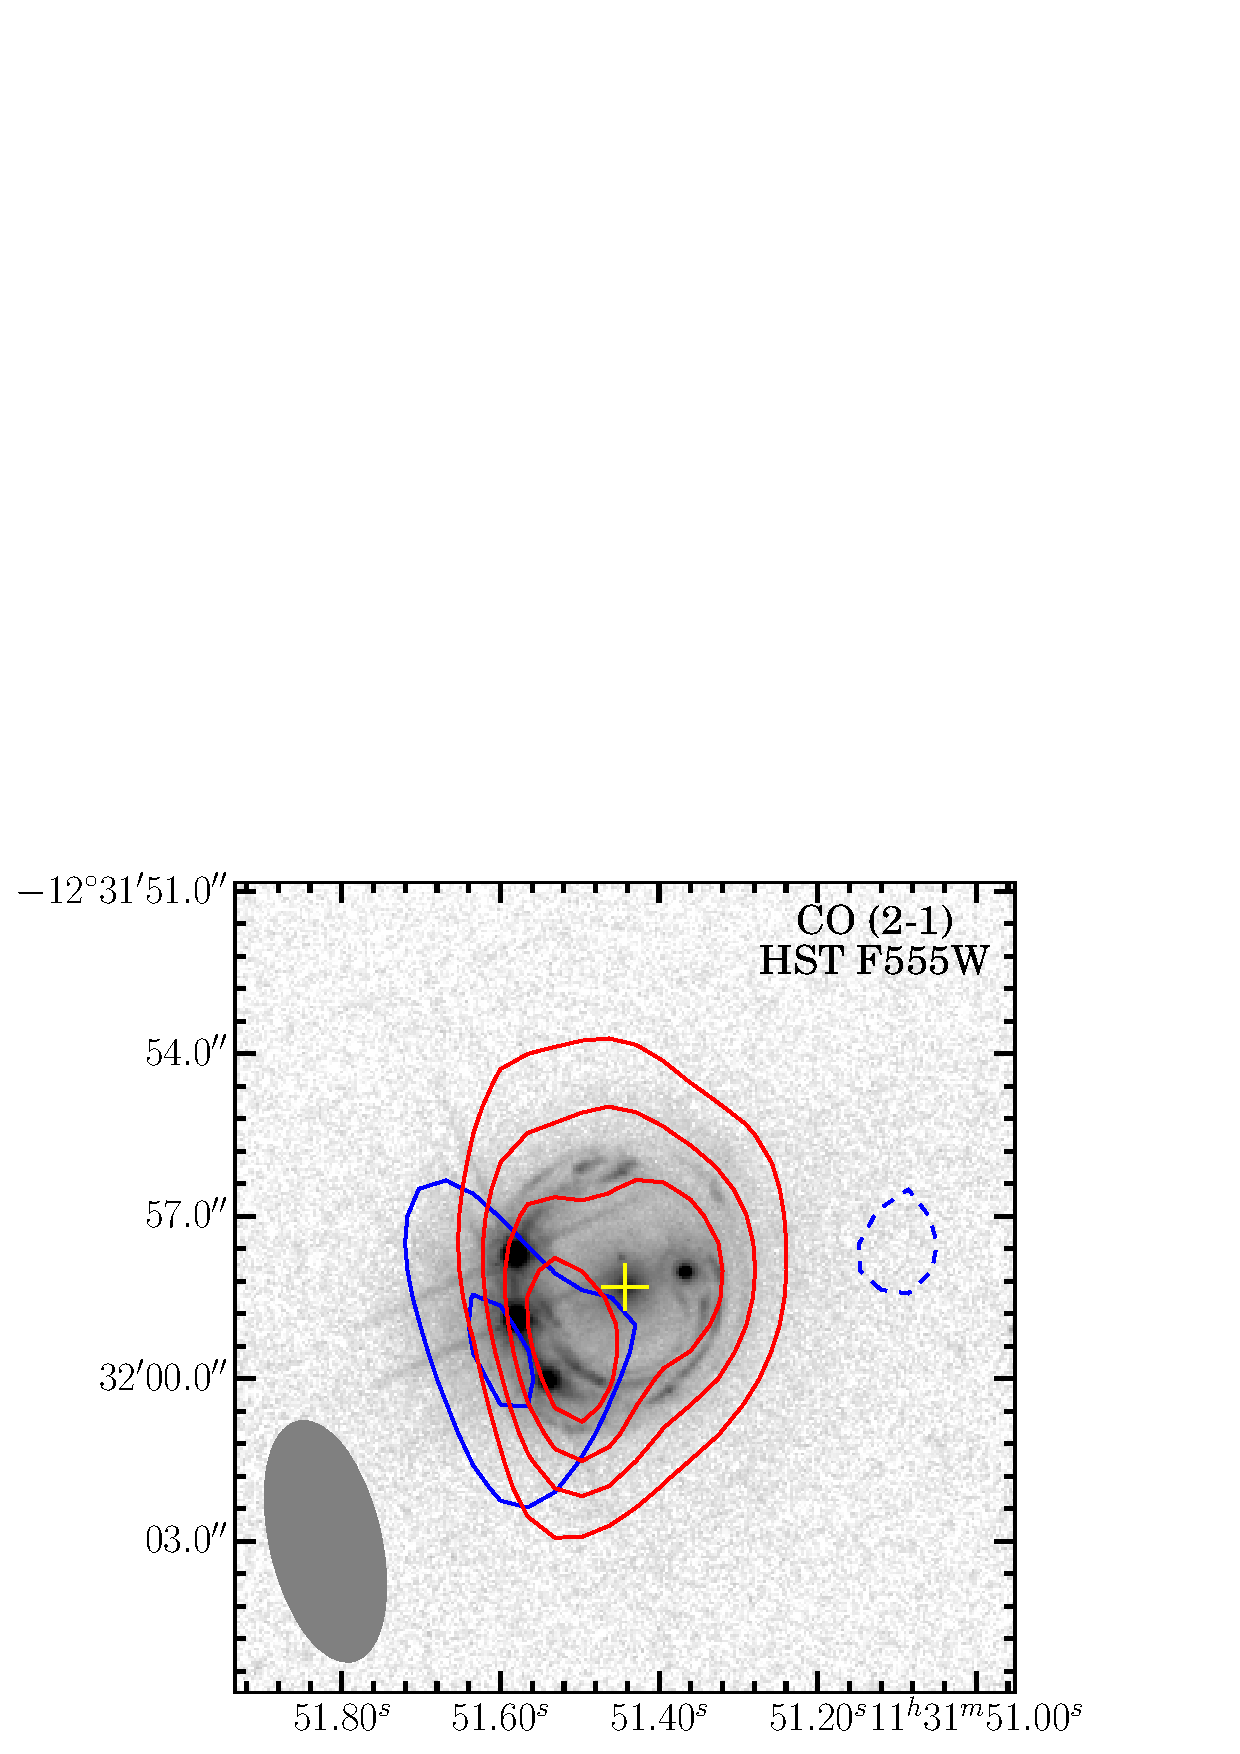
\includegraphics[width=0.25\textwidth]{../Figures/F555W_REDBLUE.png}
\includegraphics[width=0.45\textwidth]{../Figures/SpecCO21_twinx.eps}
\caption{
0th Moment map of CO(2-1) emission on HST F555W. moment-0: no clipping, of $\sigma$ 0.43 mJy beam\pmOne.
Spectrum. Velocity scale w.r.t z=0.6537
 \label{fig:CO21mom0}}
\end{figure*}


\begin{figure}[tbph]
\centering
\includegraphics[width=0.5\textwidth]{../Figures/CO_highOmom_CLIP5sigma}
\caption{
1st and 2nd order moments, clipped at 5 $\sigma$. 1st moment contour steps of 50 \kms, 2nd moment steps of 100 \kms.
velocity range in z=0 frame = [-530.33, 72.73] \kms
chan = [127, 155]
sigma = 0.16821825 Jy \kms per Beam
theshold: 5*sigma = 7.2550e-3 Jy per beam (per channel)
 \label{fig:highOmoments}}
\end{figure}




\begin{figure*}[tbph]
\centering
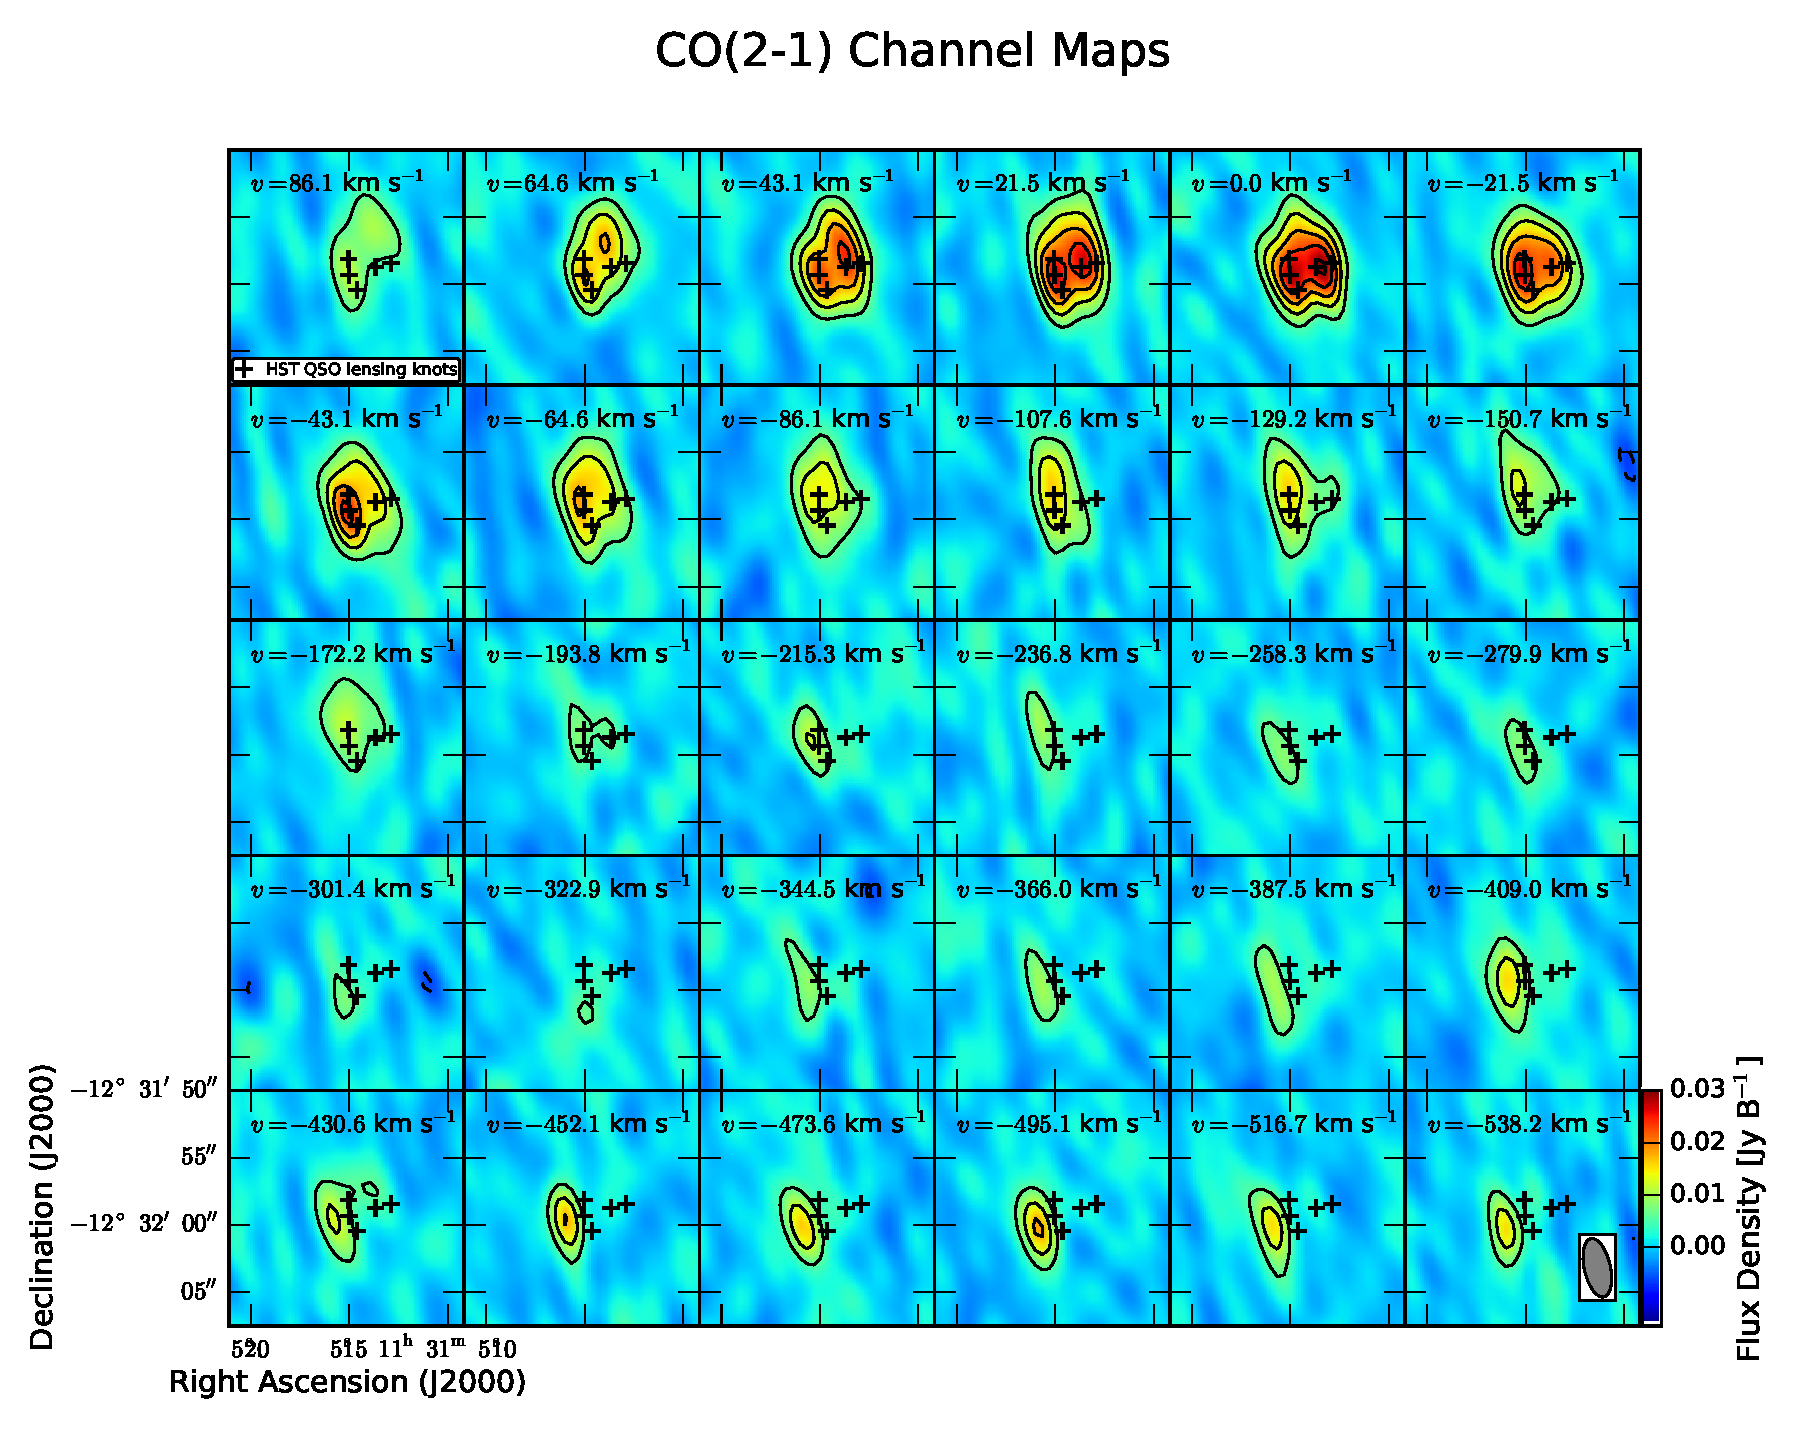
\includegraphics[width=0.8\textwidth]{../Figures/co_channel_maps.eps}	 %
\caption{
Black crosses indicate the position of the lensed AGN (components ABCD) and the central white-filled star indicates the
position of the foreground lensing galaxy (component G) as detected in the HST image. Contours $\pm$ 3$\sigma$
 \label{fig:chanmap}}
\end{figure*}

\begin{figure*}[tbph]
\centering
\includegraphics[width=0.8\textwidth]{../Figures/spatialSpec_offsetShifted.eps}
\caption{
Spatial spectra, binned by 3 pixels in each direction (1\farcs5)
 \label{fig:spatialSpec}}
\end{figure*}



\section{Interferometric Continuum}
%%%%%%%%%%%%%%%%%%%%%%%%%%%%%%%%%%%%%
% PdBI
% 2mm continuum averaged over chan 1 120 165 360
% number of channels = 316
% sigma = 1.451 mJy/B / sqrt(316) = 0.081625 mJy/B
% go noise on map (whole map) after cleaning: 89.274 µJy/B
% F = 1.2 mJy (integrated spatially, from ~ 1 sigma contour; 150 pixels)
%
%
%%%%%%%%%%%%%%%%%%%%%%%%%%%%%%%%%%%%%%%%
% VLA C Band
%

VLA C Band continuum image shows resolved jets and core emission from the foreground lensing galaxy as well as the 
background
lensed quasar (as arcs). We extracted the 5GHz fluxes for the arcs and the core as listed in Table \ref{tab:photometry}.

As shown in Figure \ref{fig:cont}, we detect 2mm continuum emission toward both the foreground galaxy and the background 
as lensed
emission.
The integrated continuum flux density is 1.2 mJy, while the peak emission is centered on the foreground galaxy at 
$S_\nu$ of 8 \micron Jy beam\pmOne.  The detection is hence marginally resolved along one axis as shown in Figure \ref{fig:contco21}.
We extract the background emission by subtracting the foreground emission as modeled by a point source (since source is 
unresolved).
After subtracting the peak, rms is same as before.
Consistency checked: the peak in the residual coincide with previous potential emission from arc, also the peak flux in the 
residual is 0.389 mJy.
The flux in the residual after removing a point source model is just consistent with the difference between the integrated and 
the peak in the
image plane, which we adopt as continuum in the background source at 2mm, which is $\sim$ 0.4 mJy.

We fit power law to the VLA C band radio data and the 2mm continuum, we derive a spectral index of $\alpha$=0.025.
\begin{figure}[!htbp]
\centering
\includegraphics[width=0.3\textwidth]{../Figures/ContCO21.eps}
\caption{CO 21 moment0 overlay on 2mm continuum.  % chan [127,155]
TODO: add the beam
 \label{fig:contco21}}
\end{figure}

\begin{figure}[!htbp]
\centering
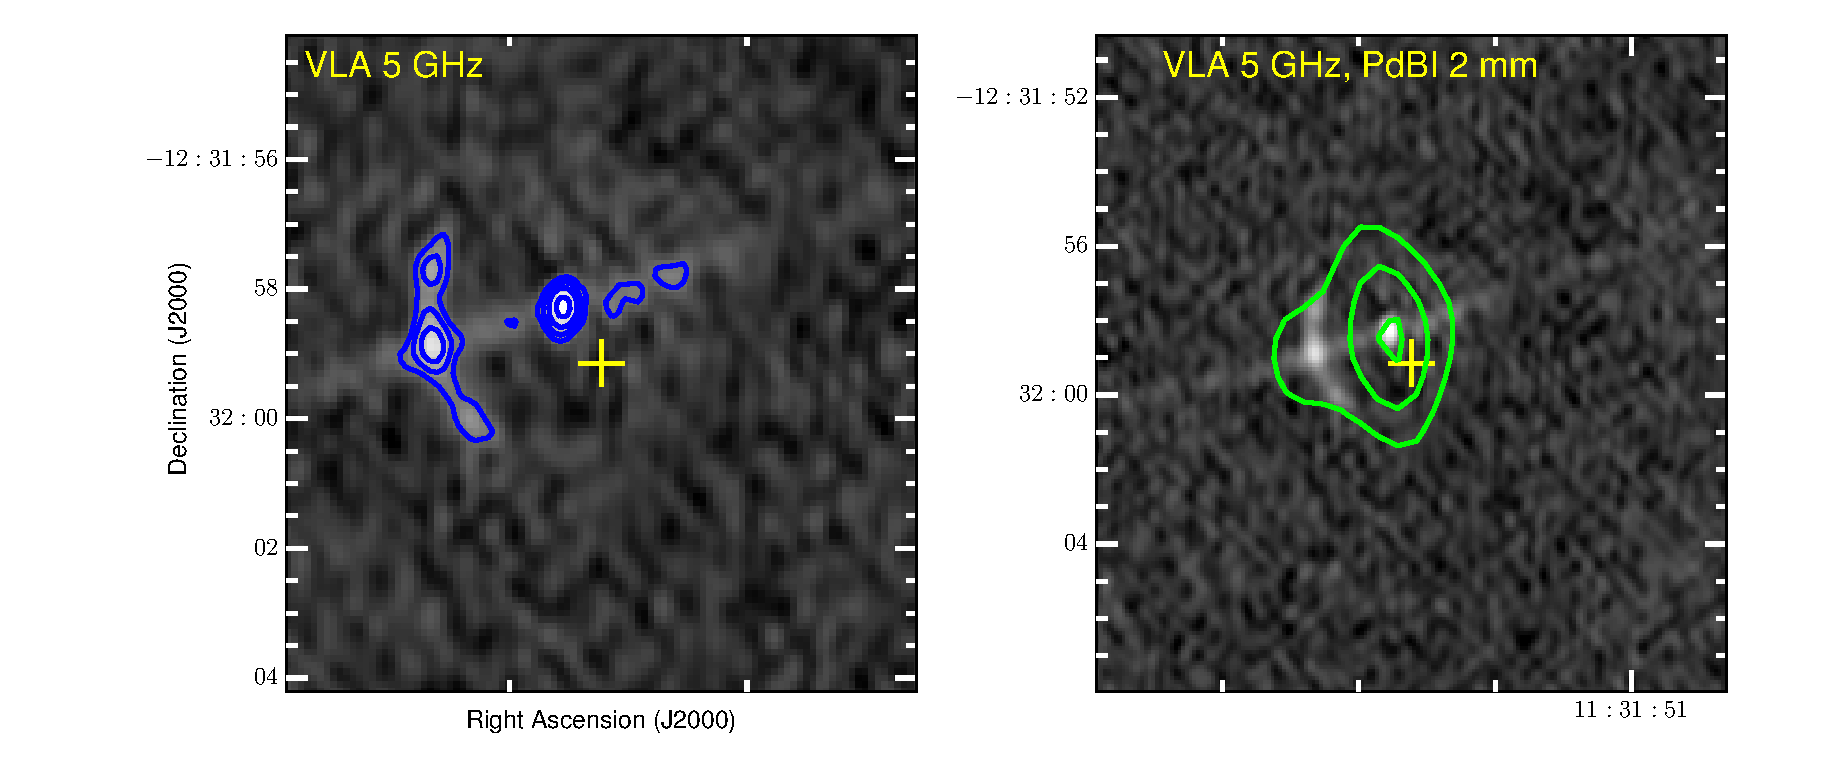
\includegraphics[width=0.8\textwidth]{../Figures/Cont2mm_5GHz_double.eps}
\caption{VLA 5GHz continuum and PdBI 2mm continuum
 \label{fig:cont}}
\end{figure}


\begin{figure}[!htbp]
\centering
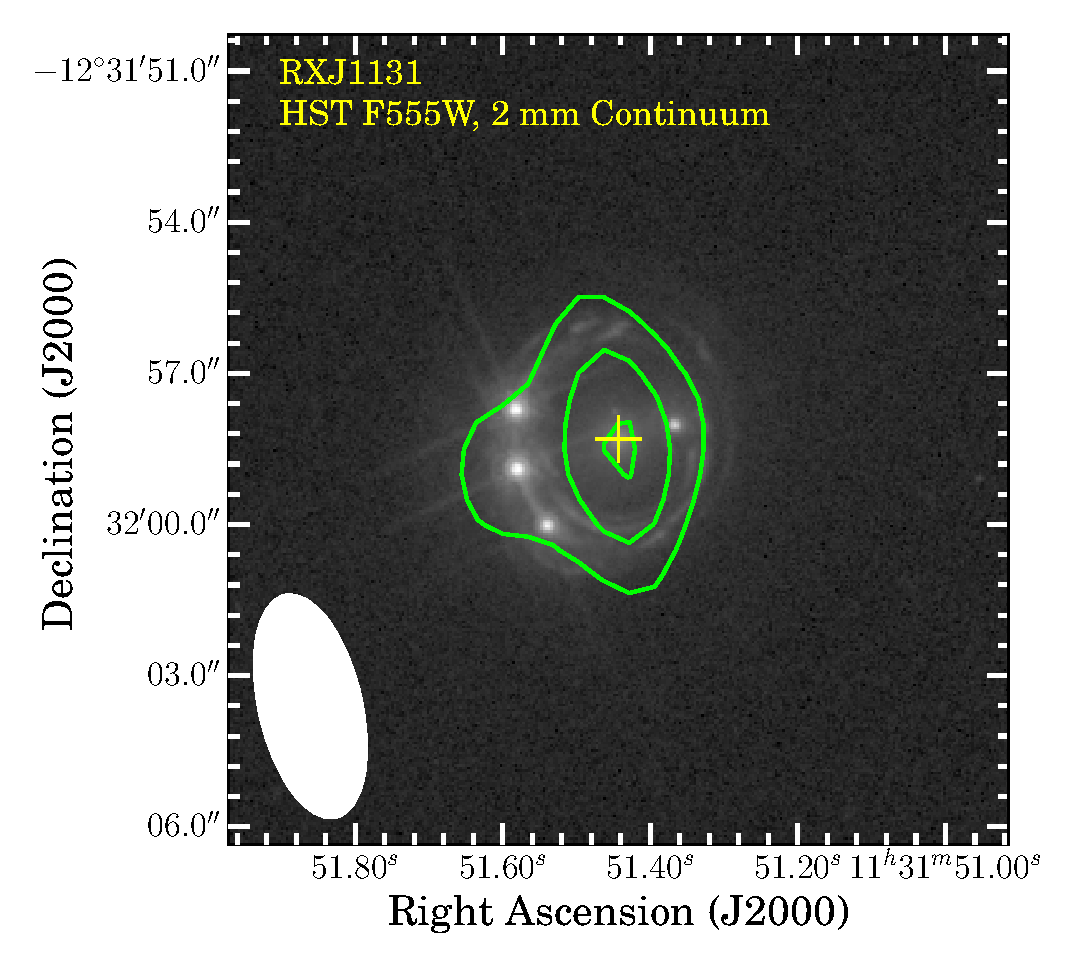
\includegraphics[width=0.35\textwidth]{../Figures/F555W_ContPdBI.eps}
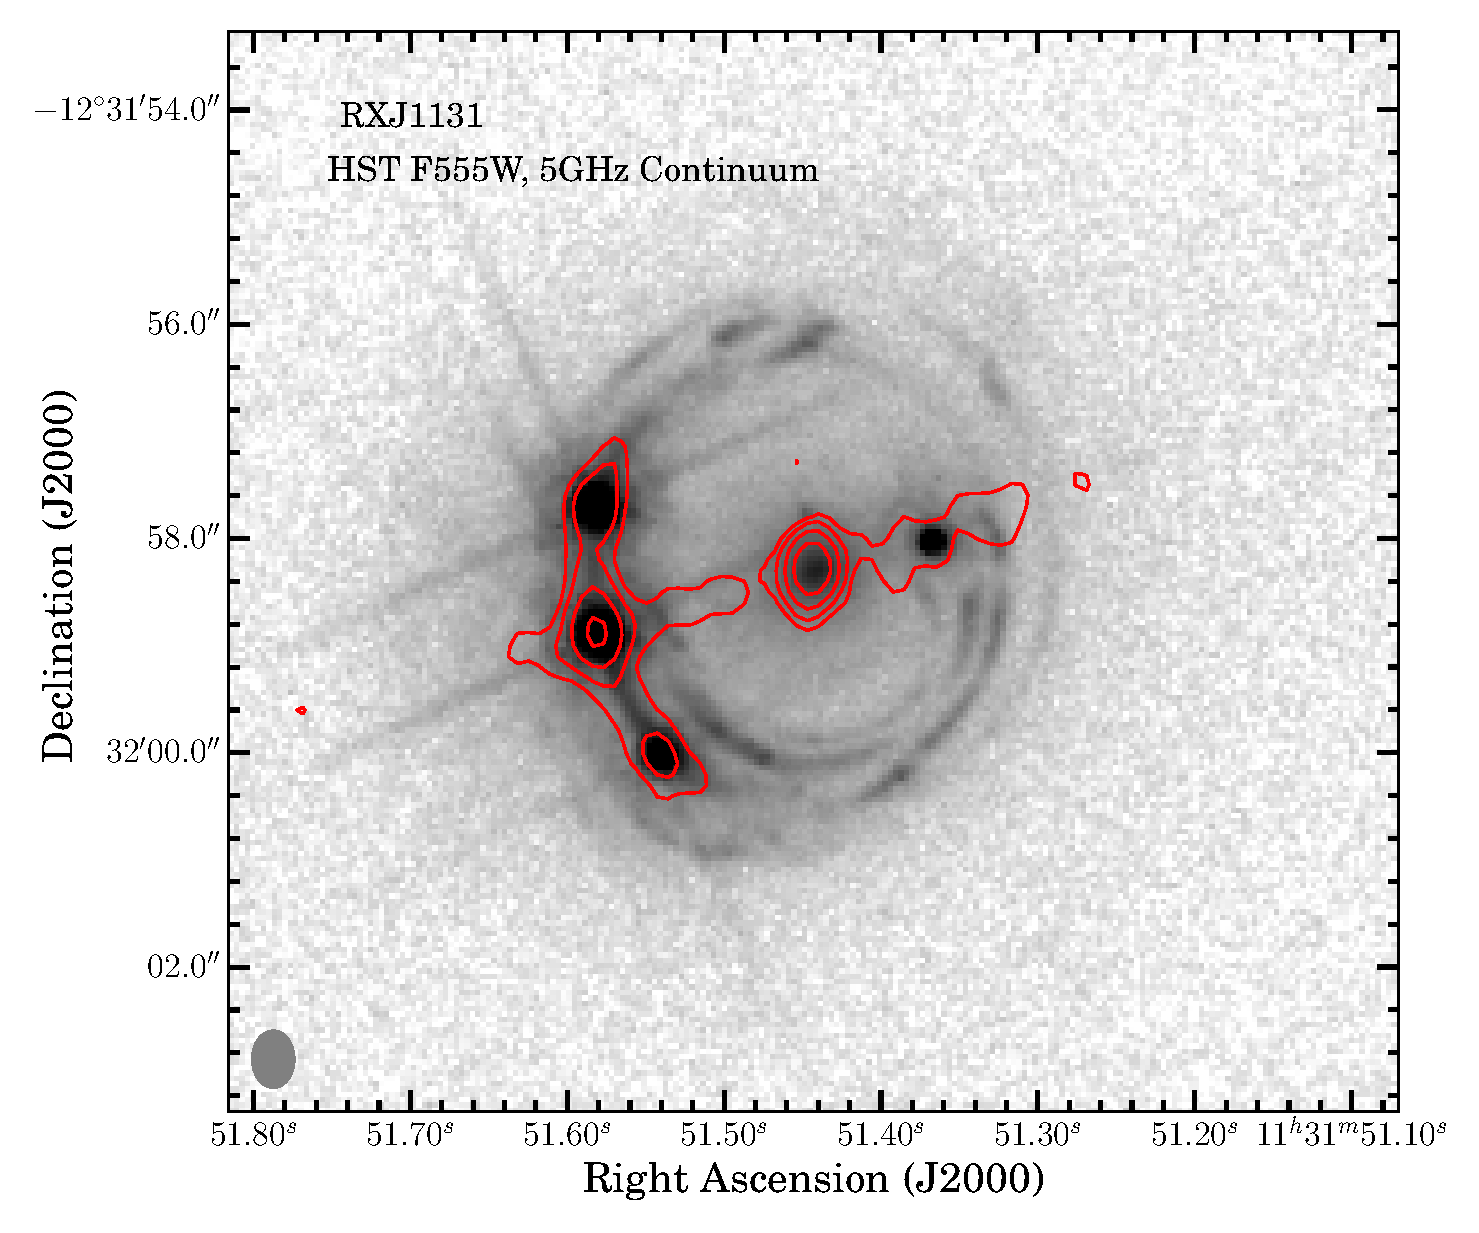
\includegraphics[width=0.35\textwidth]{../Figures/F555W_ContVLA.eps}
\caption{
can kill left figure eventually by combining this to ContCO21.eps
Right: alignment of HST and VLA 5 GHz continuum
 \label{fig:}}
\end{figure}


\section{gas kinematics and dynamics}
% data 1st moment map:
the observed velocity fields represents the rotation velocities.  
We note that the velocity field is likely affected by
systematic errors and by beam smearing given the spatial resolution of our data.

The magnitude of the
effect of beam smearing thus depends on the combination of
the size of the beam, the distribution of the gas, the inclination
angle of the galaxy and the velocity gradients.

Before evaluating the rotation curve, beam smearing is taken into account. CO Gas emission is smeared out due to the finite 
beam size of the telescope. This causes shallower gradients in the velocity field, which makes the inner part of the rotation 
curve (generally where it has the steepest gradient in a disk) less steep/with shallower gradients.  
The inner part of the rotation curve is most affected by beam smearing; as this is 
where the curve is changing the most, you need more points to accurately connect them. 

 To correct for beam smearing, a model curve (data cubes?) was chosen and then a beam smear term was added to match the observed 
rotation curve. Construct a set of model galaxies with known input rotation curves and convolve with beam to match 
observations. Then, derive rotation curve by fitting tilted rings to the intensity-weighted mean velocity field.

fit to a set of PV diagram

\subsection{Dynamical Lens model of \rot{2}{1}}
We construct a two-dimensional map of the velocity field in the source plane using the \rot{2}{1} emission. 
The source-plane velocity field is shown in Figure \ref{fig:blah} and resembles a rotating 

% Interpretation of the lens model
- C06 suggest the presence of an interacting dusty galaxy in their HST
observations, which BJB+08 calls it the F component. The lensed images of the
ABCDE
components coincide with our CO data (see mom0 on HST and channel map),
evidently CO emission coming from the AGN host galaxy.
- one of the red channels in our lens model suggests a second source component,
which is consistent with the spatially offset dusty source (see mom0 on HST,
which
the red velocity component coincides with this F component)

%%%%%%%%%%%%%%%%%%%%%%%%
We compare our lens model parameters on the mass distribution of the lensing
galaxy with literature, particularly against the SIE model presented by C06.
In C06, their SIE model shows position of lensing mass is offset by (-0.015",
-0.041" from obsservations (i.e. light centroid)); PA = -73.6, ellipticity = 0.45,
theta\_R = 1.84" $\pm$ 0.01.
Our best-fit model parameters finds a BLAH
	- Our model lens parameters (median):
		- file: serenity/model/src/medianLens0Param.dat
		- lensing gal. position is consistent with C06,
		- Einstein radius: consistent with C06
		- PA: consistent within errors
		- Axial ratio: consistent within errors
%%%%%%%%%%%%%%%%%%%%%%%%%

Differential lensing is at play as suggested by the spectral shape of the \rot{2}{1} line profile, where
flux density in the red wing is much high than in the blue wing.
We modelled the emission using different kinematic components, the magnification factors are reported in Table BLAH.
\begin{deluxetable}{lccc}[!htbp]
\tabletypesize{\scriptsize}
\tablecolumns{3}
\tablecaption{\rot{2}{1} Magnification factors.}
\tablehead{
\colhead{channel} & 
\colhead{Source 1 $\mu_{\rm L}$} & 
\colhead{Source 2 $\mu_{\rm L}$} & 
}
\startdata
126-130 & 7.2 $\pm$ 5.6 & 6.7 $\pm$ 2.5 \\ %which is source 1 and 2 then?
131-135 & 7.6 $\pm$ 1.6 & \\ % would this be source 1 or 2?
136-140 & 8.7 $\pm$ 2.0 & \\
141-145 & 4.1 $\pm$ 0.9 & \\
146-150 & 4.2 $\pm$ 0.6 & \\
151-156 & 4.3 $\pm$ 2.4 & \\
156-160 & 3.1 $\pm$ 0.9 & \\
weighted average & 4.4 & \\
median & 5.5 &  \\
\enddata
\label{tab:mag}
\tablecomments{blah}
 %TablenotegoesBetween 
\tablerefs{blah}
\end{deluxetable}


\begin{figure*}[tbph]
\centering
\includegraphics[width=0.85\textwidth]{../Figures/PostageStampModel.eps}
\includegraphics[width=0.85\textwidth]{../Figures/PostageStampResiduals.eps}
\caption{
of channel widths $\sim$ 100\kms.
\label{fig:}}
\end{figure*}


%%%%%%%%%%%%%%%%%%%%%%%%%%%%%%%%%%%%%%%%%%
\section{SED}

\subsection{Photometry}

We obtain archival and published photometry.
2MASS magnitudes from the 2MASS All-Sky
Catalog of Point SourcesBLAH  (Skrutskie et al. 2006), WISE magnitudes
from the AllWISE Source CatalogBLAH, Spitzer/MIPS
data from BLAH Catalog, IRAS photometry from the IRAS point source
and faint source cataloguesBLAH.

The Herschel/SPIRE data are from the Herschel Science Archive, processed
by the SPIRE HIPE pipeline version 12BLAH (Ott 2010). The
photometry was extracted at the source position using the
SUSSEXTractor task within HIPE (Savage \& Oliver 2007,
Smith et al 2012, Pearson et al 2014). The SUSSEXtractor
task estimates the flux density from an image smoothed with
a convolution kernel derived from the SPIRE beam FWHM.
The flux density measured by SUSSEXtractor
was verified using the SPIRE Timeline Fitter (Bendo et
al. 2013) which fits a two dimensional elliptical Gaussian
function at the source position in the timeline data. The
agreement between the SUSSEXtractor and Timeline Fitter
flux densities was found to be better than $\sim$BLAH per cent.

We list the mid-IR to FIR photometries compiled from 2MASS, WISE,IRAS, IRAC catalogs in Table \ref{fig:photometry}.

We fit SED models to the photometry of dust emission in RXJ1131-1231 with a power-law attached to the blue side.
We include the IRAS 60\micron and 100\micron upper limits to constrain the dust peak.
We also fit SED models including the 24.0\micron data from Spitzer/MIPS. 


\begin{figure*}[tbph]
\centering
\includegraphics[width=0.8\textwidth]{../Figures/FullSED.eps}
\caption{TODO: change sym indicating the VLA data, (now two points at the same frequency), change sym for the 2 points on 
2mm
PdBI (now integrated and peak), extract flux after removing a point source model.
Note THAT the WISE flux is higher than the IRAC data, probably just due to the smaller aperture used in Spitzer flux 
extraction.
Spitzer IRAC: Aperture flux in 5\farcs diameter with aperture correction applied. Spitzer/MIPS: PSF fit flux, as source size < 
native PSF
FWHM of 6".
Might want to add NVSS constraints.
 \label{fig:}}
\end{figure*}

\begin{deluxetable}{lccc}[!htbp]
\centering
\tabletypesize{\scriptsize}
\tablecolumns{4}
\tablecaption{Photometry data}
\tablehead{\colhead{Wavelength} & \colhead{Frequency} & \colhead{Flux Density} & \colhead{Instrument}\\
\colhead{($\micron$)} & \colhead{(GHz)} & \colhead{(mJy)} & \colhead{ } \vspace{0.05in}
\\  \cline{1-4} \vspace{-0.05in} \\
\multicolumn{4}{c}{Combined/Unresolved}
}
\startdata
1.25    & 239834  & 1.009 $\pm$ 0.09    & CTIO/J-Band \\
1.65    & 181692  & 1.448 $\pm$ 0.12    & CTIO/H-Band \\
2.17    & 138153  & 2.064 $\pm$ 0.16    & CTIO/Ks-Band \\
3.4     & 88174.2 & 7.027 $\pm$ 0.14    & {\it WISE}/W1 \\
3.6     & 83275.7 & 5.618 $\pm$ 0.0021  & {\em Spitzer}/IRAC \\
4.5     & 66620.5 & 7.803 $\pm$ 0.0021  & {\em Spitzer}/IRAC \\
4.6     & 65172.3 & 8.872 $\pm$ 0.16    & {\it WISE}/W2 \\
5.8     & 51688.4 & 10.720 $\pm$ 0.0051 & {\it Spitzer}/IRAC \\
8.0     & 37474.1 & 14.470 $\pm$ 0.0041 & {\it Spitzer}/IRAC \\
12      & 24982.7 & 21.960 $\pm$ 0.42   & {\it WISE}/W3 \\
12      & 24982.7 & $<$400              & {\it IRAS} \\
22      & 13626.9 & 55.110 $\pm$ 1.9    & {\it WISE}/W4 \\
24      & 12491.4 & 70.204 $\pm$ 0.026  & {\it Spitzer}/MIPS \\
25      & 11991.7 & $<$ 500             & {\it IRAS} \\
60      & 4996.54 & $<$ 600             & {\it IRAS} \\
100     & 2997.92 & $<$ 1000            & {\it IRAS} \\
250     & 1199.17 & 289.4 $\pm$ 9.6     & {\it Herschel}/SPIRE \\
350     & 856.55  & 168.2 $\pm$ 8.6     & {\it Herschel}/SPIRE \\
500     & 599.585 & 56.8 $\pm$ 8.8      & {\it Herschel}/SPIRE \\
1387.93 & 216     & $<$2.492            & CARMA \\
2152.82 & 139.256 & 1.230 $\pm$ 0.220   & PdBI \\
\cutinhead{Foreground Lensing Galaxy (deblended bands)} \\ [-1.5ex]
0.555   & 540167  & 0.056 $\pm$ 0.006   & {\it HST}-ACS/V-Band \\
0.814   & 368295  & 0.238 $\pm$ 0.013   & {\it HST}-ACS/I-Band \\
1.6     & 187370  & 0.539 $\pm$ 0.041   & {\it HST}-NICMOS(NIC2)/H-Band \\
3.6     & 83275.7 & 0.585 $\pm$ 0.003\tna   & {\em Spitzer}/IRAC \\
4.5     & 66620.5 & 1.794 $\pm$ 0.0027\tna  & {\em Spitzer}/IRAC \\
5.8     & 51688.4 & 3.163 $\pm$ 0.0059\tna  & {\it Spitzer}/IRAC \\
8.0     & 37474.1 & 4.589 $\pm$ 0.0057\tna  & {\it Spitzer}/IRAC \\
2152.82 & 139.256 & 0.799 $\pm$ 0.082   & PdBI \\
61414   & 4.8815  & 0.866 $\pm$ 0.027   & VLA \\
\cutinhead{Background Galaxy RXJ1131 (deblended bands)}
0.555   & 540167  & 0.009 $\pm$ 0.0041\tnb  & {\it HST}-ACS/V-Band \\
0.814   & 368295  & 0.041 $\pm$ 0.0054\tnb  & {\it HST}-ACS/I-Band \\
1.6     & 187370  & 0.133 $\pm$ 0.004\tnb   & {\it HST}-NICMOS(NIC2)/H-Band \\
3.6     & 83275.7 & 5.034 $\pm$ 0.0021  & {\em Spitzer}/IRAC \\
4.5     & 66620.5 & 6.009 $\pm$ 0.0017  & {\em Spitzer}/IRAC \\
5.8     & 51688.4 & 7.557 $\pm$ 0.003   & {\it Spitzer}/IRAC \\
8.0     & 37474.1 & 9.881 $\pm$ 0.0039  & {\it Spitzer}/IRAC\\
2152.82 & 139.256 & 0.400 $\pm$ 0.082\tnc   & PdBI \\
61414   & 4.8815  & 1.273 $\pm$ 0.042   & VLA
\enddata
\label{tab:photometry}
\tablecomments{The IRAC photometry for channel 1 (3.6\,$\micron$) is extracted directly from the image and
from the Spitzer Heritage Archive for channels 2$-$4 (4.5, 5.8, and 8.0\,$\micron$). All upper limits are 3$\sigma$.}
\tablenotetext{a}{Flux obtained using aperture photometry after subtracting the emission of RXJ1131 from the total emission.}
\tablenotetext{b}{A contribution from the quasar has been removed (see C06), and thus the flux density corresponds to the host galaxy only.}
\tablenotetext{c}{Flux extracted from the residual map after subtracting a point-source model.}
\tablerefs{The {\it HST} photometry is adopted from C06.}
\end{deluxetable}



  %--------------------------------------------------------------------------
  %                              Conclusion
  %--------------------------------------------------------------------------
\section{Discussion and conclusions}
We observed the cold molecular gas properties using CO line emission toward the AGN host galaxy RXJ1131-1231 at 
$z_{\rm CO}$\,$\sim$BLAH. 
Fitting SED models, we find that the AGN host galaxy is a ULIRG. 
A faint companion as seen in HST observations (BJB) is also detected in our CO, confirming it's redshift and gas rich nature.

%==============================================================================
%                                Back matters
%==============================================================================


% ACKNOWLEDGEMENTS
%-----------------
\acknowledgments
We thank...

  %--------------------------------------------------------------------------
  %                               Bibliography
  %--------------------------------------------------------------------------
\bibliographystyle{yahapj}
\bibliography{RXJ.bib}
\end{document}